\section{PTC thermistors}
As aforementioned, a positive temperature coefficient thermistor (also called \textbf{posistor}) is a thermally sensitive resistor that varies its resistivity as the temperature of the environment changes. Particularly because it is a positive coefficient, as the temperature increases, the resistivity of the semiconductor device increases as well.

\subsection{Charateristics}
One of the most important properties of the PTC thermistor is the characteristic curve between the \textbf{resistance} $R$ and the \textbf{temperature} $T$, which has to be converted from Celsius (or Fahrenheit) to Kelvin. Its curve is a positive exponential graph that respects the following equation \cite{Saburi196353}:

\begin{equation*}
    R = R_0\,e^{\beta\,(\frac{1}{T} - \frac{1}{T_0})}
\end{equation*}

\noindent Where $R$ is the calculated resistance at the temperature $T$ and $R_0$ is the resistance measured at temperature $T_0$. The coefficient $\beta$ is the thermistor constant and it depends on the materials used to build it and on the thermistor dimensions. It is possible to obtain this value by measuring its resistance value at two different temperatures and computing the following equation \cite{Saburi196353}.

\begin{equation*}
    \beta = \frac{\ln{\frac{R_2}{R_1}}}{\frac{1}{T_2} - \frac{1}{T_1}}
\end{equation*}

\noindent Using the previous equations, the curve can be plotted by writing down the equations using MATLAB, or other programming languages. Figure \ref{fig:PTC_logarithmic} shows how much the resistance increases as the temperature increases. In this case, the coefficient $\beta$ has been calculated by assuming that when $T_1 = 273.15 K$, $R_1 = 1k\Omega$ and when $T_2 = 373.15 K$, $R_2 = 100M\Omega$.\footnote{Please be aware that the selected values are purely for illustrative purposes; no devices with these characteristics exist in reality}

\begin{figure}[h]
    \centering
    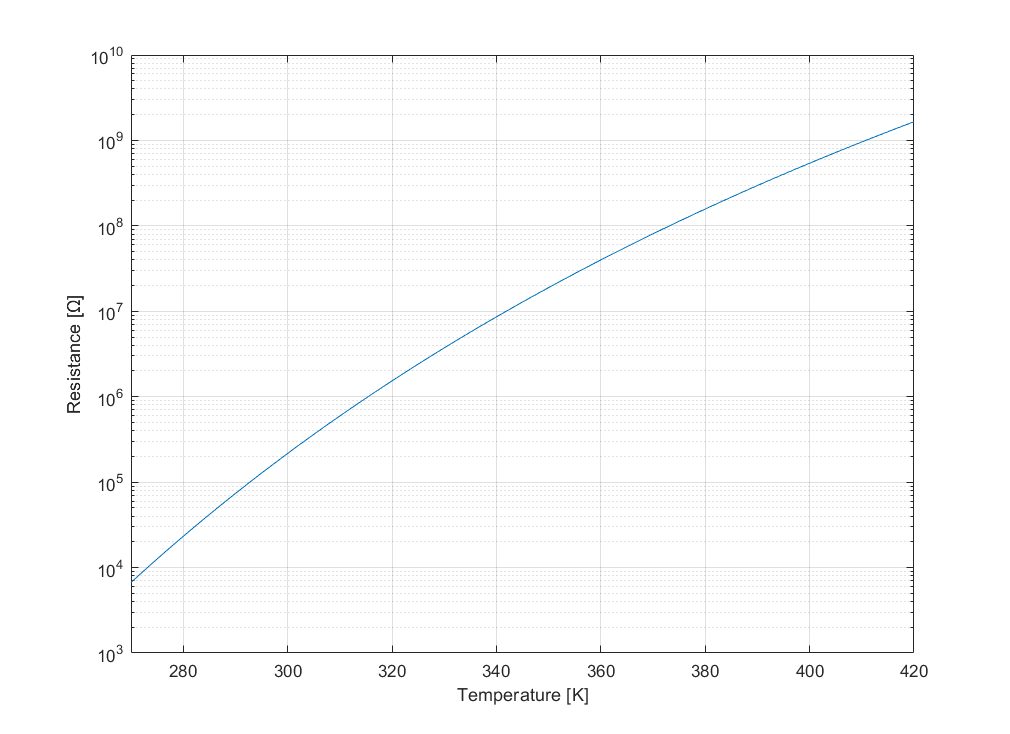
\includegraphics[width = .7\textwidth]{../res/plots/PTC_logarithmic.png}
    \label{fig:PTC_logarithmic}
    \caption{PTC resistance-temperature logarithmic curve.}
\end{figure}

\FloatBarrier\noindent Secondly it might be interesting to plot the change ratio between the resistance $R$ and the value of the resistance at some fixed temperature. In the figure \ref{fig:PTC_ratio}, the fixed temperature value $T_0$ was 25° celsius (or 298.15 Kelvin) which implies that $R_0 = 16.7 k\Omega$.

\begin{figure}[h]
    \centering
    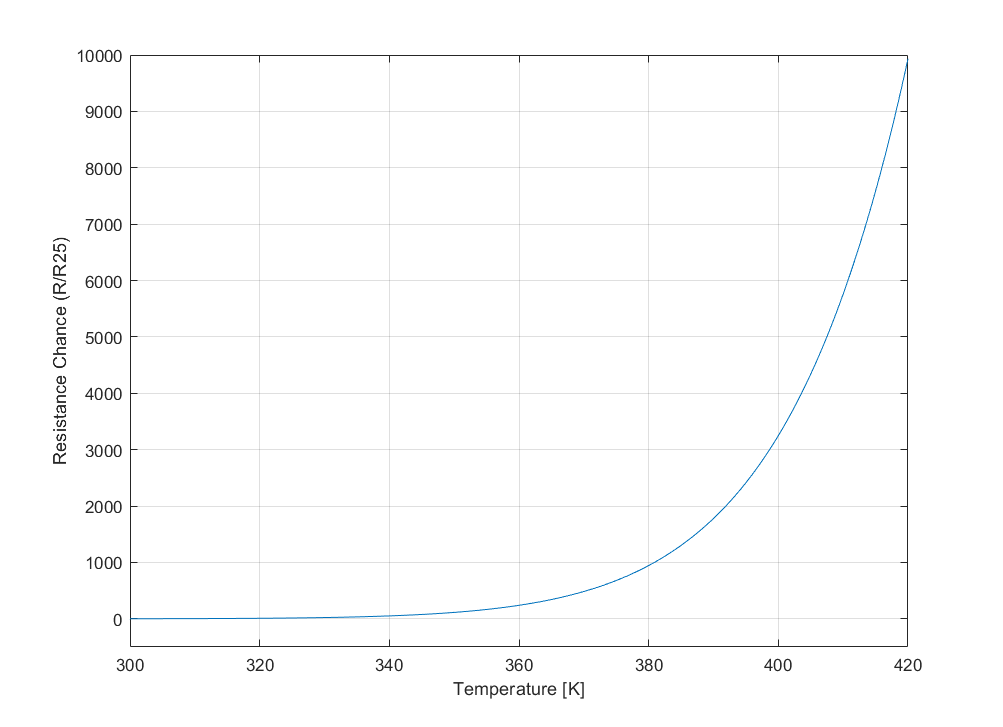
\includegraphics[width = .7\textwidth]{../res/plots/PTC_ratio.png}
    \label{fig:PTC_ratio}
    \caption{PTC change ratio between $R$ and $R_0$}
\end{figure}

\FloatBarrier\noindent In both of the plots the resistance value or the change ratio drastically increases as the environment gets hotter. In the next paragraph, we will see how important this characteristic is for building current-regulating circuits and protecting delicate components.

Another important coefficient to know about is the \textbf{dissipation constant} $\delta$ which describes the power needed to increase the thermistor temperature by 1° Celsius through self-heating. The dissipation constant varies on the construction materials of the thermistor and the environment \cite{Saburi196353}. The constant $\delta$ is useful to describe the power dissipation of the thermistor when its temperature is $T$ (at thermal equilibrium) and the ambient temperature is $T_0$:

\begin{equation*}
    P = VI = \delta(T - T_0)
\end{equation*}

\noindent By knowing the power dissipation it is then possible to plot the \textbf{current-voltage} relationship when the PTC thermistor is in a state of thermal equilibrium. Sure enough, by knowing the constant $\delta$ and the room temperature $T_0$, the power dissipation $P$ can be obtained and then it is possible to calculate the voltage and the current relationship:

\begin{equation*}
    V = \sqrt{P \cdot R} \hspace{50px} I = \sqrt{\frac{P}{R}}
\end{equation*}

\noindent By setting $\delta = 4.5 mW/^{\circ}C$ and the room temperature $T_0 = 25^{\circ}C = 298.15^{\circ} K$, it is possible to plot some important relationship. Figure \ref{fig:PTC_curr-temp} describes the relationship between the current and the temperature in the PTC thermistor: as the temperature increases the current decreases; this is because when the temperature increases, also the resistance increases and, as such, the current flowing through will reasonably decrease.

\begin{figure}[h]
    \centering
    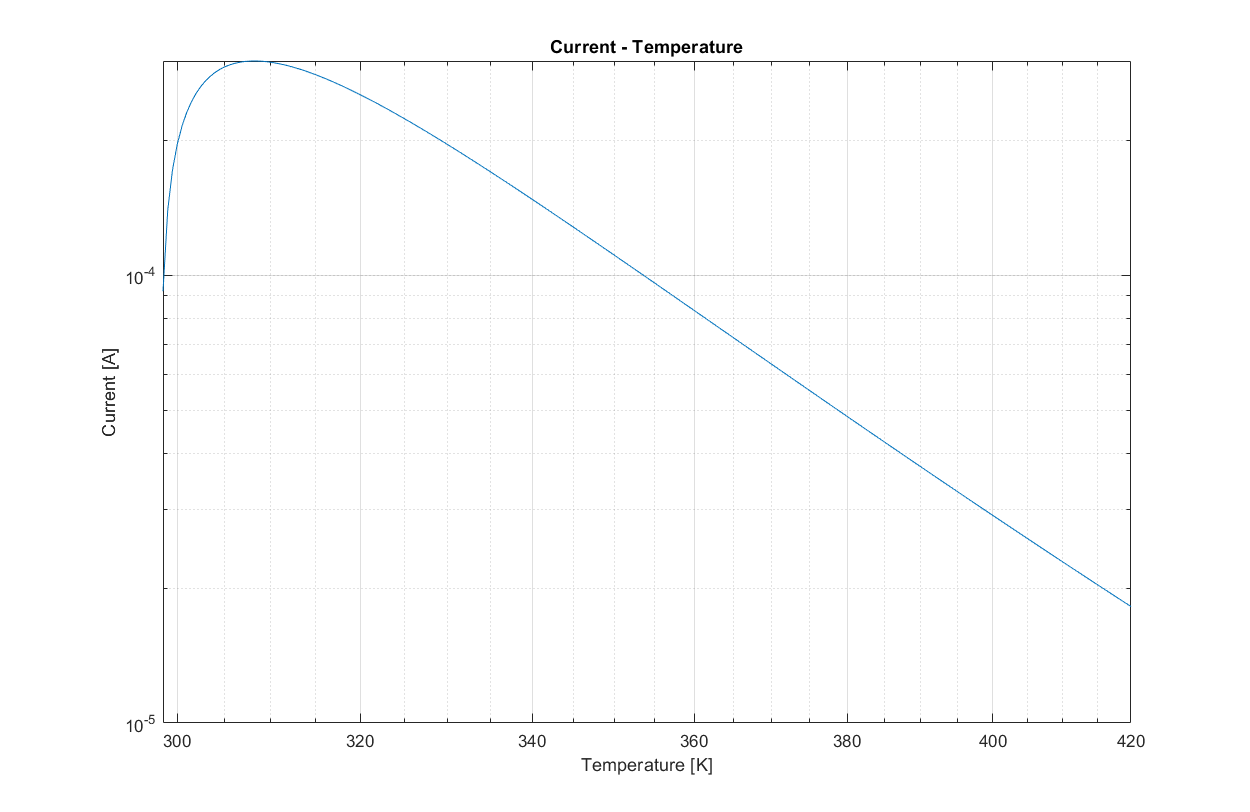
\includegraphics[width = .7\textwidth]{../res/plots/PTC_curr-temp.png}
    \label{fig:PTC_curr-temp}
    \caption{Corrent-temperature relationship of a PTC thermistor.}
\end{figure}

\FloatBarrier \noindent The relationship between the temperature and the voltage is shown in the image \ref{fig:PTC_volt-temp}. Contrarily to the current-temperature relationship, here, as the temperature increases, the voltage of the thermistor rises as well because its resistivity intensifies.

\begin{figure}[h]
    \centering
    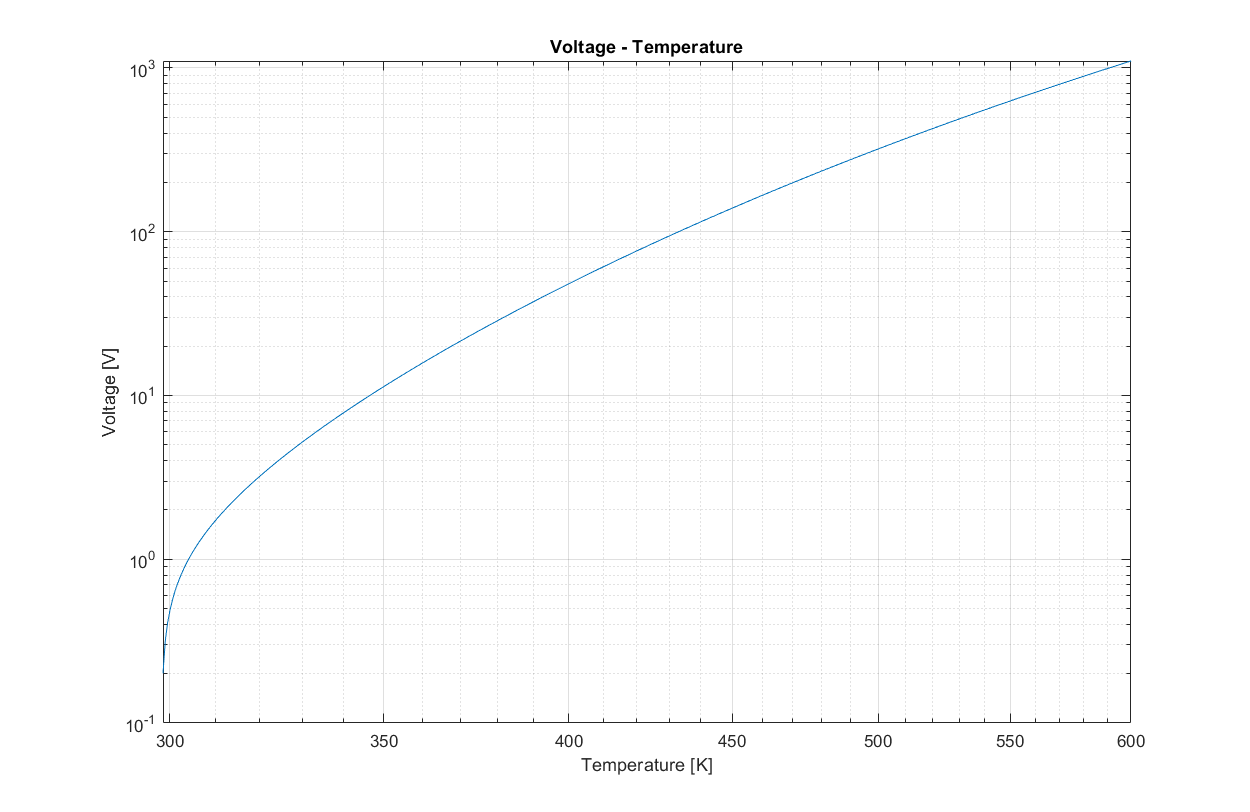
\includegraphics[width = .7\textwidth]{../res/plots/PTC_volt-temp.png}
    \label{fig:PTC_volt-temp}
    \caption{Voltage-temperature relationship of a PTC thermistor.}
\end{figure}

\FloatBarrier \noindent In the figure \ref{fig:PTC_curr-volt} there is the characteristic curve current-voltage of the PTC thermistor. The plot is an \textsl{insofar} curve: when the slope is positive there is a constant-resistance state meanwhile when the slope of the curve is negative there is a constant-power range \cite{Saburi196353}.

\begin{figure}[h]
    \centering
    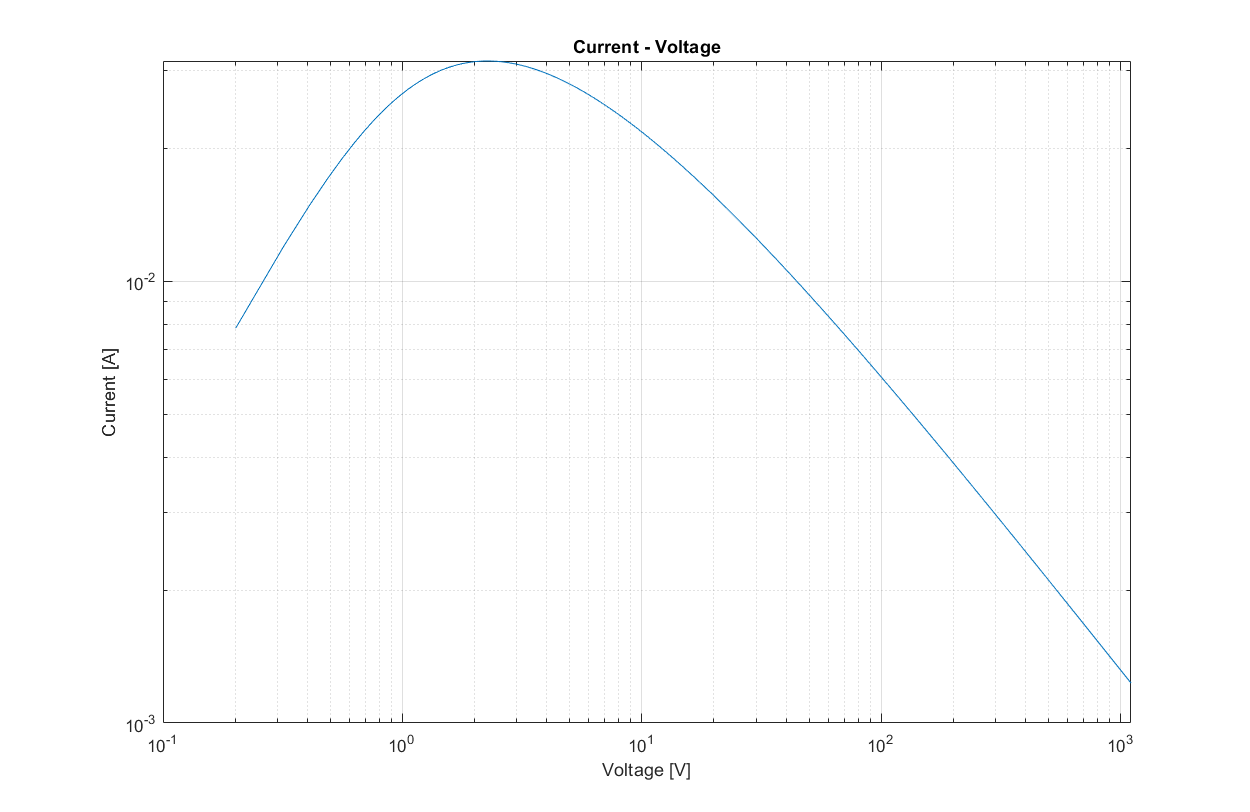
\includegraphics[width = .7\textwidth]{../res/plots/PTC_curr-volt.png}
    \label{fig:PTC_curr-volt}
    \caption{Current-voltage relationship of a PTC thermistor.}
\end{figure}

\FloatBarrier \subsection{Applications}





